\subsection{Интеграция ИИ-модуля DeepSeek в архитектуру проекта}

Для обеспечения эффективной работы ИИ-компонента в образовательной платформе реализована модульная архитектура с чётким разделением ответственности. Последующие подразделы детализируют ключевые аспекты интеграции: стратегию контейнеризации для изоляции сервиса, механизмы взаимодействия с клиентской частью и системные преимущества выбранного подхода. Основное внимание уделено сохранению прозрачности работы ИИ для конечных пользователей при обеспечении гибкости разработки и эксплуатации.

\subsubsection{Контейнеризация DeepSeek}
Для обеспечения независимого жизненного цикла и лёгкой масштабируемости ИИ-компонента DeepSeek развёртывается в виде изолированного Docker-контейнера. Такой подход позволяет:

\begin{enumerate}
  \item Быстро запускать и останавливать сервис без влияния на основное приложение;
  \item Поддерживать разные версии DeepSeek параллельно, экспериментируя с обновлениями моделей;
  \item Мигрировать между хостами и облачными средами с минимальными изменениями конфигурации.
\end{enumerate}

\subsubsection{Преимущества контейнеризированного подхода}
Контейнеризация DeepSeek даёт следующие ключевые плюсы:
\begin{enumerate}
  \item Анализ текста программы выполняется в отдельном окружении, не влияя на отзывчивость интерфейса;
  \item При большом числе запросов можно запускать несколько экземпляров контейнера;
  \item Обновление ИИ-компонента сводится к выпуску нового образа без правок в клиентской части;
  \item Контейнеры можно запускать локально и в облаке с одинаковой конфигурацией.
\end{enumerate}

\subsubsection{Взаимодействие клиентской части с DeepSeek}

Клиентская часть приложения, реализованная на React и Next.js, отправляет HTTP-запросы к серверной части веб-приложения при прикреплении решения задания студентом, далее автоматический начинается проверка решения при помощи анализ на основе искусственного интеллекта. Результат проверки приходит пользователю при запросе на получения детальной информации по задаче, выполненной студентом.

\begin{figure}[h]
    \centering
    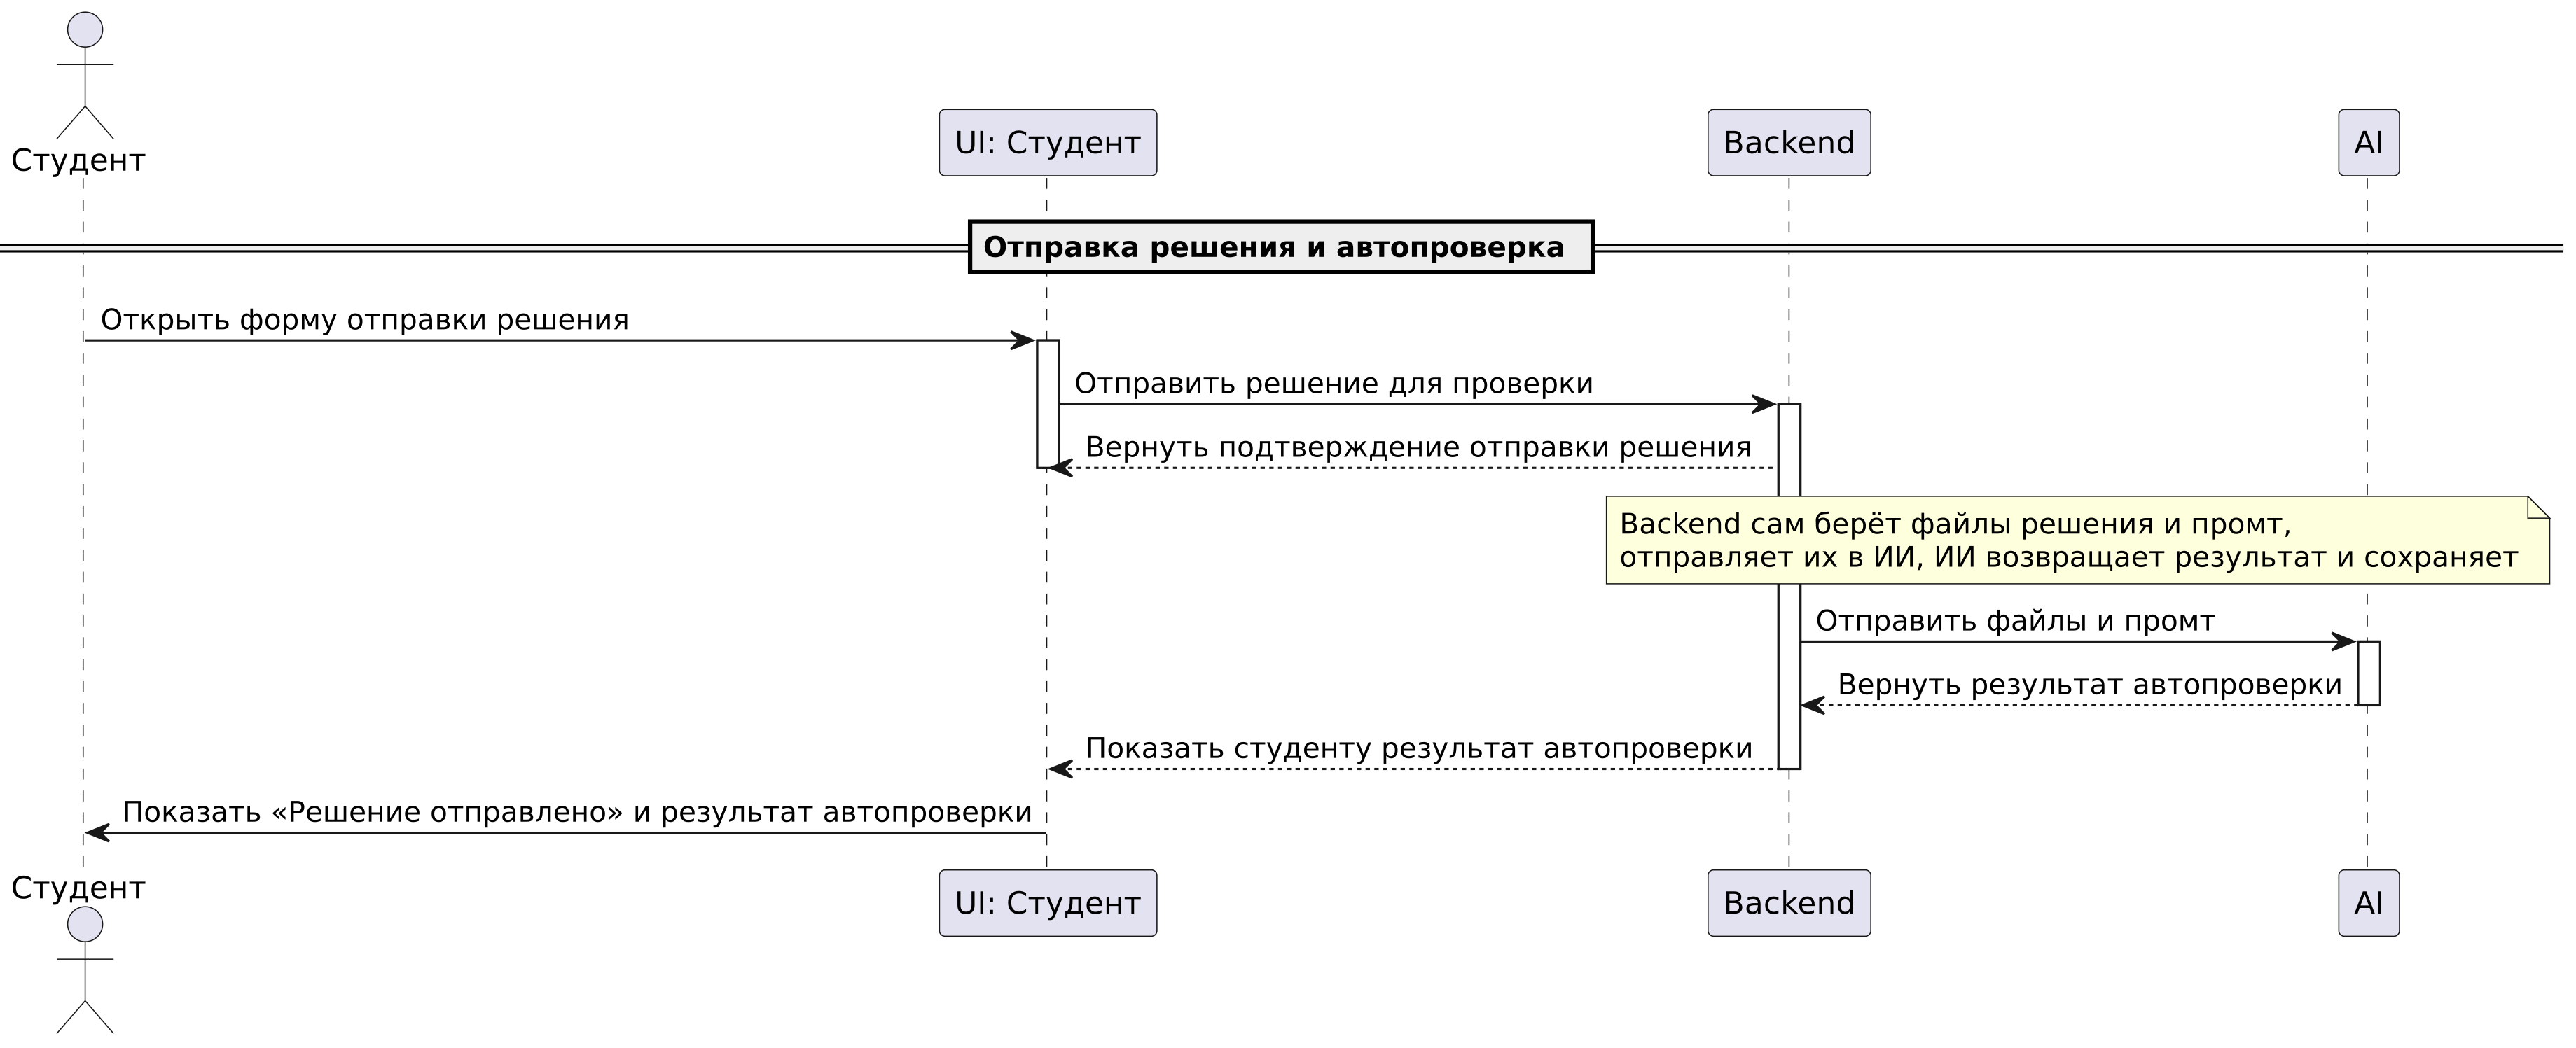
\includegraphics[width=0.8\linewidth]{static/diagrams/TaskSendStudentDiagram.png}
    \caption{Схема взаимодействия клиентской части (React/Next.js) с модулем DeepSeek}
    \label{fig:client-deepseek}
\end{figure}

На рисунке \ref{fig:client-deepseek} представлена схема взаимодействия клиентской части с модулем DeepSeek.

\subsubsection{Вывод}

Контейнеризация DeepSeek обеспечивает полную независимость остальных компонентов приложения от ИИ-модуля, позволяя развёртывать и обновлять его без влияния на другие сервисы. Взаимодействие через API сервера создаёт своего рода «чёрный ящик» для клиента, что упрощает инкапсуляцию логики и даёт гибкость в распределении и масштабировании нагрузки на контейнер с ИИ.


